% Options for packages loaded elsewhere
\PassOptionsToPackage{unicode}{hyperref}
\PassOptionsToPackage{hyphens}{url}
%
\documentclass[
]{article}
\usepackage{amsmath,amssymb}
\usepackage{lmodern}
\usepackage{iftex}
\ifPDFTeX
  \usepackage[T1]{fontenc}
  \usepackage[utf8]{inputenc}
  \usepackage{textcomp} % provide euro and other symbols
\else % if luatex or xetex
  \usepackage{unicode-math}
  \defaultfontfeatures{Scale=MatchLowercase}
  \defaultfontfeatures[\rmfamily]{Ligatures=TeX,Scale=1}
\fi
% Use upquote if available, for straight quotes in verbatim environments
\IfFileExists{upquote.sty}{\usepackage{upquote}}{}
\IfFileExists{microtype.sty}{% use microtype if available
  \usepackage[]{microtype}
  \UseMicrotypeSet[protrusion]{basicmath} % disable protrusion for tt fonts
}{}
\makeatletter
\@ifundefined{KOMAClassName}{% if non-KOMA class
  \IfFileExists{parskip.sty}{%
    \usepackage{parskip}
  }{% else
    \setlength{\parindent}{0pt}
    \setlength{\parskip}{6pt plus 2pt minus 1pt}}
}{% if KOMA class
  \KOMAoptions{parskip=half}}
\makeatother
\usepackage{xcolor}
\usepackage[margin=1in]{geometry}
\usepackage{color}
\usepackage{fancyvrb}
\newcommand{\VerbBar}{|}
\newcommand{\VERB}{\Verb[commandchars=\\\{\}]}
\DefineVerbatimEnvironment{Highlighting}{Verbatim}{commandchars=\\\{\}}
% Add ',fontsize=\small' for more characters per line
\usepackage{framed}
\definecolor{shadecolor}{RGB}{248,248,248}
\newenvironment{Shaded}{\begin{snugshade}}{\end{snugshade}}
\newcommand{\AlertTok}[1]{\textcolor[rgb]{0.94,0.16,0.16}{#1}}
\newcommand{\AnnotationTok}[1]{\textcolor[rgb]{0.56,0.35,0.01}{\textbf{\textit{#1}}}}
\newcommand{\AttributeTok}[1]{\textcolor[rgb]{0.77,0.63,0.00}{#1}}
\newcommand{\BaseNTok}[1]{\textcolor[rgb]{0.00,0.00,0.81}{#1}}
\newcommand{\BuiltInTok}[1]{#1}
\newcommand{\CharTok}[1]{\textcolor[rgb]{0.31,0.60,0.02}{#1}}
\newcommand{\CommentTok}[1]{\textcolor[rgb]{0.56,0.35,0.01}{\textit{#1}}}
\newcommand{\CommentVarTok}[1]{\textcolor[rgb]{0.56,0.35,0.01}{\textbf{\textit{#1}}}}
\newcommand{\ConstantTok}[1]{\textcolor[rgb]{0.00,0.00,0.00}{#1}}
\newcommand{\ControlFlowTok}[1]{\textcolor[rgb]{0.13,0.29,0.53}{\textbf{#1}}}
\newcommand{\DataTypeTok}[1]{\textcolor[rgb]{0.13,0.29,0.53}{#1}}
\newcommand{\DecValTok}[1]{\textcolor[rgb]{0.00,0.00,0.81}{#1}}
\newcommand{\DocumentationTok}[1]{\textcolor[rgb]{0.56,0.35,0.01}{\textbf{\textit{#1}}}}
\newcommand{\ErrorTok}[1]{\textcolor[rgb]{0.64,0.00,0.00}{\textbf{#1}}}
\newcommand{\ExtensionTok}[1]{#1}
\newcommand{\FloatTok}[1]{\textcolor[rgb]{0.00,0.00,0.81}{#1}}
\newcommand{\FunctionTok}[1]{\textcolor[rgb]{0.00,0.00,0.00}{#1}}
\newcommand{\ImportTok}[1]{#1}
\newcommand{\InformationTok}[1]{\textcolor[rgb]{0.56,0.35,0.01}{\textbf{\textit{#1}}}}
\newcommand{\KeywordTok}[1]{\textcolor[rgb]{0.13,0.29,0.53}{\textbf{#1}}}
\newcommand{\NormalTok}[1]{#1}
\newcommand{\OperatorTok}[1]{\textcolor[rgb]{0.81,0.36,0.00}{\textbf{#1}}}
\newcommand{\OtherTok}[1]{\textcolor[rgb]{0.56,0.35,0.01}{#1}}
\newcommand{\PreprocessorTok}[1]{\textcolor[rgb]{0.56,0.35,0.01}{\textit{#1}}}
\newcommand{\RegionMarkerTok}[1]{#1}
\newcommand{\SpecialCharTok}[1]{\textcolor[rgb]{0.00,0.00,0.00}{#1}}
\newcommand{\SpecialStringTok}[1]{\textcolor[rgb]{0.31,0.60,0.02}{#1}}
\newcommand{\StringTok}[1]{\textcolor[rgb]{0.31,0.60,0.02}{#1}}
\newcommand{\VariableTok}[1]{\textcolor[rgb]{0.00,0.00,0.00}{#1}}
\newcommand{\VerbatimStringTok}[1]{\textcolor[rgb]{0.31,0.60,0.02}{#1}}
\newcommand{\WarningTok}[1]{\textcolor[rgb]{0.56,0.35,0.01}{\textbf{\textit{#1}}}}
\usepackage{graphicx}
\makeatletter
\def\maxwidth{\ifdim\Gin@nat@width>\linewidth\linewidth\else\Gin@nat@width\fi}
\def\maxheight{\ifdim\Gin@nat@height>\textheight\textheight\else\Gin@nat@height\fi}
\makeatother
% Scale images if necessary, so that they will not overflow the page
% margins by default, and it is still possible to overwrite the defaults
% using explicit options in \includegraphics[width, height, ...]{}
\setkeys{Gin}{width=\maxwidth,height=\maxheight,keepaspectratio}
% Set default figure placement to htbp
\makeatletter
\def\fps@figure{htbp}
\makeatother
\setlength{\emergencystretch}{3em} % prevent overfull lines
\providecommand{\tightlist}{%
  \setlength{\itemsep}{0pt}\setlength{\parskip}{0pt}}
\setcounter{secnumdepth}{-\maxdimen} % remove section numbering
\usepackage{booktabs}
\usepackage{longtable}
\usepackage{array}
\usepackage{multirow}
\usepackage{wrapfig}
\usepackage{float}
\usepackage{colortbl}
\usepackage{pdflscape}
\usepackage{tabu}
\usepackage{threeparttable}
\usepackage{threeparttablex}
\usepackage[normalem]{ulem}
\usepackage{makecell}
\usepackage{xcolor}
\ifLuaTeX
  \usepackage{selnolig}  % disable illegal ligatures
\fi
\IfFileExists{bookmark.sty}{\usepackage{bookmark}}{\usepackage{hyperref}}
\IfFileExists{xurl.sty}{\usepackage{xurl}}{} % add URL line breaks if available
\urlstyle{same} % disable monospaced font for URLs
\hypersetup{
  pdftitle={Matteo's First RMD File !},
  pdfauthor={Matteo Martone},
  hidelinks,
  pdfcreator={LaTeX via pandoc}}

\title{Matteo's First RMD File !}
\author{Matteo Martone}
\date{2022-10-28}

\begin{document}
\maketitle

\hypertarget{collatz-conjecture}{%
\subsection{Collatz Conjecture}\label{collatz-conjecture}}

The collatz conjecture states that if you pick any number, it transform
into one by a set of two arithmetic operations. If the number selected
is odd, it will be multiplied by three, and then added by one. If the
number selected is even, it will be divided by two. Once the number
reaches one, the function stops.

What we want to know is a bit different. We want to solve for the amount
of iterations the collatz conjecture processes until the number has
reached one. For example, if we had started with five we would multiply
by three and add one to get sixteen. Then we would divide by two to get
eight, then again to get four, again to get two, and finally one. This
had five total iterations. We can call this ``stopping times''.

\begin{Shaded}
\begin{Highlighting}[]
\CommentTok{\# create a function "collatzcounter" that counts the amount of times the function takes to reach 0 }
\NormalTok{collatzcounter }\OtherTok{\textless{}{-}} \ControlFlowTok{function}\NormalTok{(n, }\AttributeTok{w =} \DecValTok{0}\NormalTok{)\{}
  \CommentTok{\# if n = 1 then stop }
  \ControlFlowTok{if}\NormalTok{ (n }\SpecialCharTok{==} \DecValTok{1}\NormalTok{) \{}
    \FunctionTok{return}\NormalTok{ (w)}
  \CommentTok{\# if n is even then divide by 2}
\NormalTok{  \} }\ControlFlowTok{else} \ControlFlowTok{if}\NormalTok{ (n }\SpecialCharTok{\%\%} \DecValTok{2} \SpecialCharTok{==} \DecValTok{0}\NormalTok{) \{ }
    \FunctionTok{collatzcounter}\NormalTok{ (}\AttributeTok{n =}\NormalTok{ n}\SpecialCharTok{/}\DecValTok{2}\NormalTok{, }\AttributeTok{w =}\NormalTok{ w }\SpecialCharTok{+} \DecValTok{1}\NormalTok{)}
  \CommentTok{\# if n is odd then multiple by 3 and add 1 }
\NormalTok{  \} }\ControlFlowTok{else}\NormalTok{ \{}
    \FunctionTok{collatzcounter}\NormalTok{ (}\AttributeTok{n =} \DecValTok{3} \SpecialCharTok{*}\NormalTok{ n }\SpecialCharTok{+} \DecValTok{1}\NormalTok{, }\AttributeTok{w =}\NormalTok{ w }\SpecialCharTok{+} \DecValTok{1}\NormalTok{)}
\NormalTok{  \}}
 
\NormalTok{\}}
\CommentTok{\#invoke the function and select number you want to find numbers of times function executes to get to 1}
\FunctionTok{collatzcounter}\NormalTok{(}\DecValTok{100}\NormalTok{)}
\end{Highlighting}
\end{Shaded}

\begin{verbatim}
## [1] 25
\end{verbatim}

\begin{Shaded}
\begin{Highlighting}[]
\CommentTok{\# give example of n when the value is 100 {-} returns 25 stopping times til 1 is reached }
\end{Highlighting}
\end{Shaded}

From this code in R we can see the amount of times a number takes to
reach one using the collatz conjecture by placing any number in place of
``n''. To see this more visually we can create a histogram that displays
all different values of n and how many iterations it will take from
zero.

\begin{Shaded}
\begin{Highlighting}[]
\CommentTok{\# create a vectorize form of collatzcounter using \textquotesingle{}n\textquotesingle{}}
\NormalTok{collatzcounterVec }\OtherTok{\textless{}{-}} \FunctionTok{Vectorize}\NormalTok{(}
  \AttributeTok{FUN =}\NormalTok{ collatzcounter,}
  \AttributeTok{vectorize.args =} \StringTok{\textquotesingle{}n\textquotesingle{}}
\NormalTok{)}
\CommentTok{\# create of histogram of new vectorized form}
\CommentTok{\# set n from 1 to 10,000 based off the stoppng time}
\FunctionTok{hist}\NormalTok{(}\AttributeTok{x =} \FunctionTok{collatzcounterVec}\NormalTok{(}\AttributeTok{n =} \DecValTok{1}\SpecialCharTok{:}\DecValTok{10000}\NormalTok{),}
     \CommentTok{\# gives heading/title}
    \AttributeTok{main =} \StringTok{"Stopping Times for Collatz Conjecture"}\NormalTok{,}
    \CommentTok{\# defines x label}
    \AttributeTok{xlab =} \StringTok{"Value of n"}\NormalTok{,}
    \CommentTok{\# defines y label}
    \AttributeTok{ylab =} \StringTok{"Interations to reach 1"}\NormalTok{,}
    \CommentTok{\# setting of x to 250 and y to 2500}
    \AttributeTok{xlim =} \FunctionTok{c}\NormalTok{(}\DecValTok{1}\NormalTok{,}\DecValTok{250}\NormalTok{),}
    \AttributeTok{ylim =} \FunctionTok{c}\NormalTok{(}\DecValTok{1}\NormalTok{,}\DecValTok{2500}\NormalTok{),}
\NormalTok{)}
\end{Highlighting}
\end{Shaded}

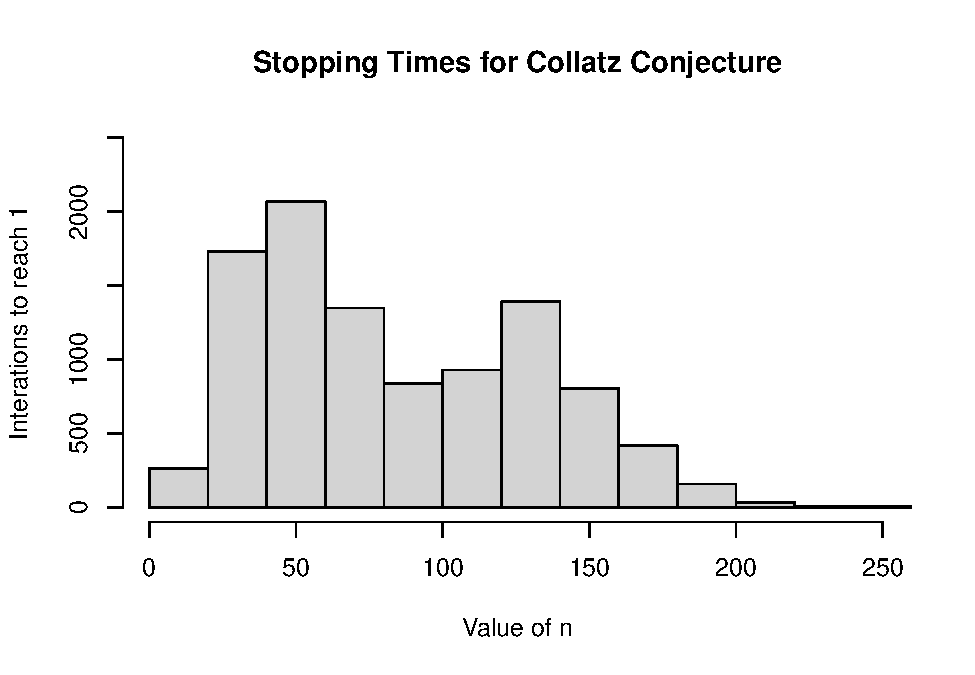
\includegraphics{Activity-8-_files/figure-latex/Histogram-1.pdf}

\hypertarget{what-can-we-learn-from-this-data-visualization}{%
\subsubsection{What can we learn from this data
visualization?}\label{what-can-we-learn-from-this-data-visualization}}

From this data visualization we can learn many things about the value of
n and the number of iterations to reach one required. We can see that
there is general downward trend of the total number of iterations
required to reach one as the value of n increases. We can see that
values of n ranging from zero to fifty are the largest, and anything
after 200 is quite minimal.

\hypertarget{diamonds}{%
\subsection{Diamonds}\label{diamonds}}

The Diamonds data set is one in which that has many different attributes
of a diamond like price, carat size, cut type, clarity and many other
sizing dimensions. From this data set there are many comparisons we can
draw up. Something interesting we can compare is the size of diamond
(measured in carats), and the price of diamond (dollars).

\begin{Shaded}
\begin{Highlighting}[]
\CommentTok{\#load packages and data}
\FunctionTok{library}\NormalTok{(ggplot2)}
\FunctionTok{data}\NormalTok{(diamonds)}

\CommentTok{\# use ggplot package to create a data visualization}
\FunctionTok{ggplot}\NormalTok{(diamonds) }\SpecialCharTok{+}
  \FunctionTok{aes}\NormalTok{(}\AttributeTok{x =}\NormalTok{ carat, }\AttributeTok{y =}\NormalTok{ price) }\SpecialCharTok{+}
  \FunctionTok{geom\_point}\NormalTok{(}
    \CommentTok{\# define shape and size of points }
    \AttributeTok{shape =} \StringTok{"diamond"}\NormalTok{,}
    \CommentTok{\#shrink size}
    \AttributeTok{size =} \FloatTok{1.25}\NormalTok{,}
    \CommentTok{\#change color to diamond like}
    \AttributeTok{colour =} \StringTok{"\#669AC6"}
\NormalTok{  ) }\SpecialCharTok{+}
  \FunctionTok{labs}\NormalTok{(}
    \CommentTok{\# add labels and title}
    \AttributeTok{x =} \StringTok{"Carat Size"}\NormalTok{,}
    \AttributeTok{y =} \StringTok{"Price"}\NormalTok{,}
    \AttributeTok{title =} \StringTok{"Diamond Price Vs Carat Size"}
\NormalTok{  ) }\SpecialCharTok{+}
  \FunctionTok{theme\_minimal}\NormalTok{()}
\end{Highlighting}
\end{Shaded}

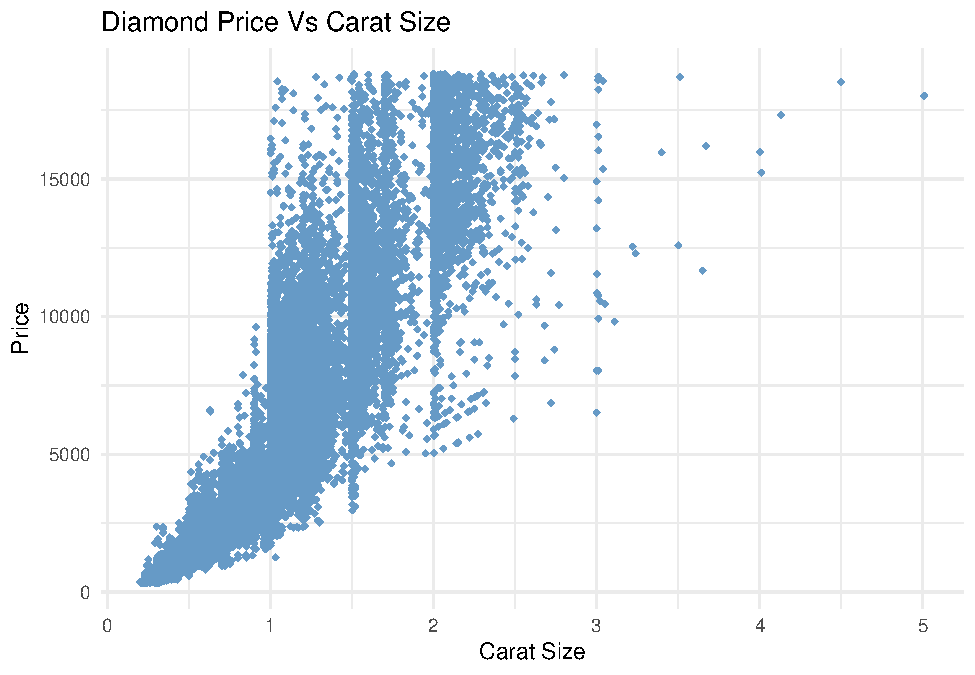
\includegraphics{Activity-8-_files/figure-latex/Diamonds - Price vs Carat Size-1.pdf}

\hypertarget{what-we-can-learn-from-this-data-visualization}{%
\subsubsection{What we can learn from this data
visualization?}\label{what-we-can-learn-from-this-data-visualization}}

From this data visualization we can immediately see a positive
correlation between carat size and the price of a diamond. We know this
because as the x-value is increasing, the y-value is as well. We can
infer that as carat size increases, price generally does as well.
However, there are many other attributes of a diamond that can have a
direct correlation to the price. The next we will be adding is the
clarity of the diamond.

\hypertarget{diamonds-data-visualization-2}{%
\subsubsection{Diamonds Data Visualization
2}\label{diamonds-data-visualization-2}}

\begin{Shaded}
\begin{Highlighting}[]
\FunctionTok{library}\NormalTok{(ggplot2)}
\FunctionTok{data}\NormalTok{(diamonds)}

\CommentTok{\# add new variable \textquotesingle{}clarity\textquotesingle{} which is defined by the color and legend}
\FunctionTok{ggplot}\NormalTok{(diamonds) }\SpecialCharTok{+}
  \FunctionTok{aes}\NormalTok{(}\AttributeTok{x =}\NormalTok{ carat, }\AttributeTok{y =}\NormalTok{ price, }\AttributeTok{color =}\NormalTok{ clarity) }\SpecialCharTok{+}
  \FunctionTok{geom\_point}\NormalTok{(}
    \AttributeTok{shape =} \StringTok{"diamond"}\NormalTok{,}
    \AttributeTok{size =} \FloatTok{1.25}\NormalTok{,}
\NormalTok{  ) }\SpecialCharTok{+} 
  \CommentTok{\# add color scaling for legend }
  \FunctionTok{scale\_color\_hue}\NormalTok{(}\AttributeTok{direction =} \DecValTok{1}\NormalTok{) }\SpecialCharTok{+}
  \FunctionTok{labs}\NormalTok{(}
    \AttributeTok{x =} \StringTok{"Carat Size"}\NormalTok{,}
    \AttributeTok{y =} \StringTok{"Price"}\NormalTok{,}
    \CommentTok{\# add new title reflecting variables }
    \AttributeTok{title =} \StringTok{"Diamond Price Vs Carat Size and Clarity"}
\NormalTok{  ) }\SpecialCharTok{+}
  \FunctionTok{theme\_minimal}\NormalTok{() }
\end{Highlighting}
\end{Shaded}

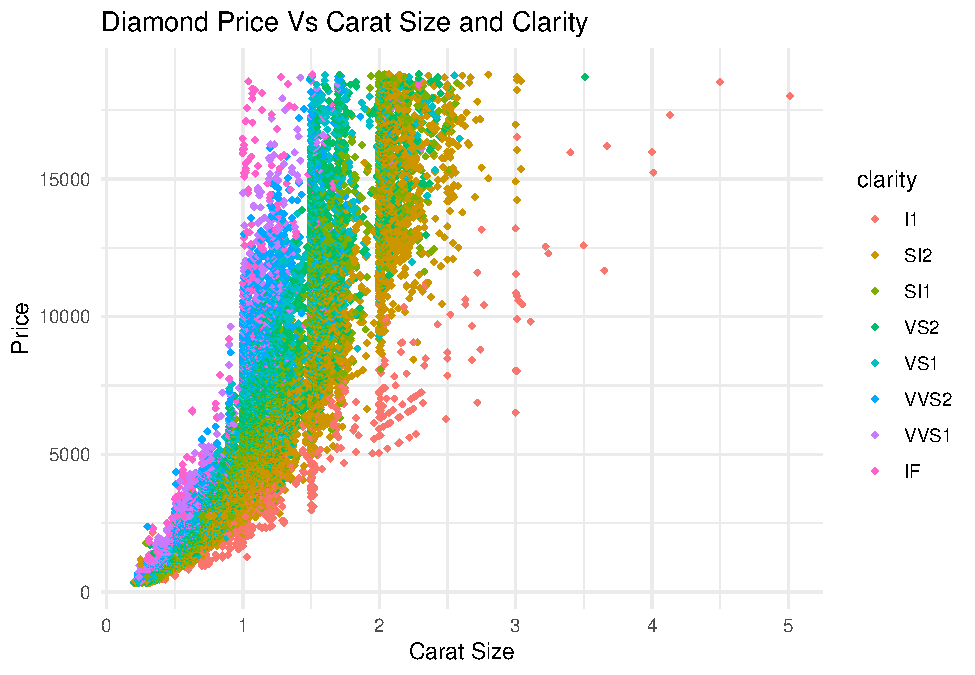
\includegraphics{Activity-8-_files/figure-latex/Diamonds - Price vs Carat Size and Clarity-1.pdf}

In the second diamonds data visualization we have a lot more to look at.
From the original we have the comparison of the carat size to price. The
next attribute we need to look at is located at the key on right side
labeled ``clarity''. Each level of clarity from I1 to IF (included to
internally flawless) is labeled by a color. When looking at the new data
visualization we can see price is heavily influence by clarity. In fact,
there is a direct correlation. When the level of clarity increases, so
does price. IF diamonds are always at the top of the pricing.

Something we can also notice is that once carat size goes beyond 2,
there seems to be a drastic decrease in IF and VVS (very very slightly
included) diamonds. This most likely has to do with the rarity. This
prove trues for other clarity as well, as carat size increases, quality
of clarity decreases in quantity.

While these two are both great comparisons to diamond price, there is
another I was to draw attention to, the cut of the diamond.

\hypertarget{diamonds-data-visualization-3}{%
\subsubsection{Diamonds data visualization
3}\label{diamonds-data-visualization-3}}

\begin{Shaded}
\begin{Highlighting}[]
\CommentTok{\#load packages and data}
\FunctionTok{library}\NormalTok{(ggplot2)}
\FunctionTok{data}\NormalTok{(diamonds)}

\CommentTok{\# add new variable \textquotesingle{}clarity\textquotesingle{} which is defined by the color and legend}
\FunctionTok{ggplot}\NormalTok{(diamonds) }\SpecialCharTok{+}
  \FunctionTok{aes}\NormalTok{(}\AttributeTok{x =}\NormalTok{ carat, }\AttributeTok{y =}\NormalTok{ price, }\AttributeTok{color =}\NormalTok{ clarity) }\SpecialCharTok{+}
  \FunctionTok{geom\_point}\NormalTok{(}
    \AttributeTok{shape =} \StringTok{"diamond"}\NormalTok{,}
    \AttributeTok{size =} \FloatTok{1.25}\NormalTok{,}
\NormalTok{  ) }\SpecialCharTok{+} 
  \CommentTok{\# add color scaling for legend }
  \FunctionTok{scale\_color\_hue}\NormalTok{(}\AttributeTok{direction =} \DecValTok{1}\NormalTok{) }\SpecialCharTok{+}
  \FunctionTok{labs}\NormalTok{(}
    \AttributeTok{x =} \StringTok{"Carat Size"}\NormalTok{,}
    \AttributeTok{y =} \StringTok{"Price"}\NormalTok{,}
    \CommentTok{\# add new title reflecting variables }
    \AttributeTok{title =} \StringTok{"Diamond Price Vs Carat Size, Clarity and Cut "}
\NormalTok{  ) }\SpecialCharTok{+}
  \FunctionTok{theme\_minimal}\NormalTok{() }\SpecialCharTok{+}
  \CommentTok{\# add facet {-}{-} new variable cut to compare each }
  \FunctionTok{facet\_wrap}\NormalTok{(}\FunctionTok{vars}\NormalTok{(cut))}
\end{Highlighting}
\end{Shaded}

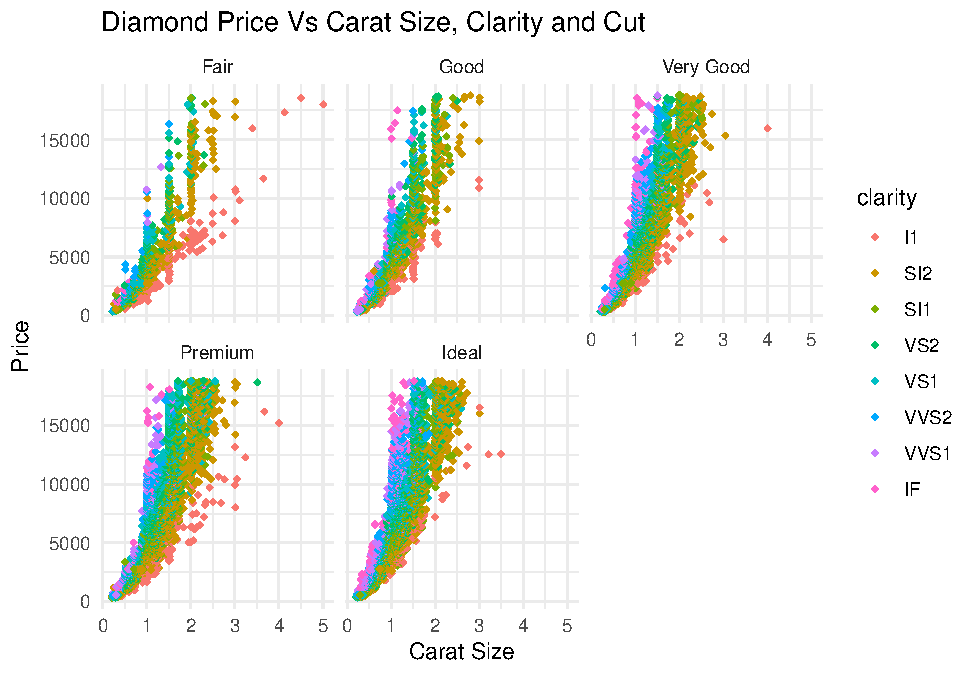
\includegraphics{Activity-8-_files/figure-latex/Diamonds - Price vs Carat size, Clarity, and Cut-1.pdf}

From this we can see the original two data visualizations. What we have
added this time is a facet to draw a greater comparison on the influence
of price. This facet creates five different visualizations with each
having respect to their own cuts (fair, good, very good, premium, and
ideal). What we can see immediately is that the cut of the diamond also
reflects to price. As cut quality increase, so does price.

We know this because of the density of the scatter plots. In the
``fair'' cut scatter plot, the correlation is positive but not super
strong. While in the ``ideal'' cut scatter plot, the correlation is
extremely positive and almost vertical. A diamond of ``ideal'' cut has
much more worth than a ``fair'' cut.

\hypertarget{diamonds-summary}{%
\subsubsection{Diamonds Summary}\label{diamonds-summary}}

Below is a summary table of the diamonds data set with respect to the
cut and width of the diamond.

\begin{Shaded}
\begin{Highlighting}[]
\CommentTok{\#load packages and data}
\FunctionTok{library}\NormalTok{(janitor)}
\end{Highlighting}
\end{Shaded}

\begin{verbatim}
## 
## Attaching package: 'janitor'
\end{verbatim}

\begin{verbatim}
## The following objects are masked from 'package:stats':
## 
##     chisq.test, fisher.test
\end{verbatim}

\begin{Shaded}
\begin{Highlighting}[]
\FunctionTok{library}\NormalTok{(dplyr) }
\end{Highlighting}
\end{Shaded}

\begin{verbatim}
## 
## Attaching package: 'dplyr'
\end{verbatim}

\begin{verbatim}
## The following objects are masked from 'package:stats':
## 
##     filter, lag
\end{verbatim}

\begin{verbatim}
## The following objects are masked from 'package:base':
## 
##     intersect, setdiff, setequal, union
\end{verbatim}

\begin{Shaded}
\begin{Highlighting}[]
\FunctionTok{library}\NormalTok{(kableExtra)}
\end{Highlighting}
\end{Shaded}

\begin{verbatim}
## 
## Attaching package: 'kableExtra'
\end{verbatim}

\begin{verbatim}
## The following object is masked from 'package:dplyr':
## 
##     group_rows
\end{verbatim}

\begin{Shaded}
\begin{Highlighting}[]
\FunctionTok{data}\NormalTok{(diamonds)}

\NormalTok{diamondsummary\_y }\OtherTok{\textless{}{-}}\NormalTok{ diamonds }\SpecialCharTok{\%\textgreater{}\%}
  \CommentTok{\#sorts all by the cut}
  \FunctionTok{group\_by}\NormalTok{(cut) }\SpecialCharTok{\%\textgreater{}\%}
  \CommentTok{\# select y which is the width }
  \FunctionTok{select}\NormalTok{(cut, y ) }\SpecialCharTok{\%\textgreater{}\%}
  \CommentTok{\# summarize function for wanted info below}
  \FunctionTok{summarize}\NormalTok{(}
    \FunctionTok{across}\NormalTok{(}
      \AttributeTok{.cols =} \FunctionTok{where}\NormalTok{(is.numeric),}
      \AttributeTok{.fns =} \FunctionTok{list}\NormalTok{(}
        \AttributeTok{min =} \SpecialCharTok{\textasciitilde{}}\FunctionTok{min}\NormalTok{(.x, }\AttributeTok{na.rm =} \ConstantTok{TRUE}\NormalTok{),}
        \CommentTok{\# even though this says quantile, they are quintile broken up by there prob {-} .2.4.6.8}
        \AttributeTok{Q1 =} \SpecialCharTok{\textasciitilde{}}\FunctionTok{quantile}\NormalTok{(.x, }\AttributeTok{probs =} \FloatTok{0.2}\NormalTok{, }\AttributeTok{na.rm =} \ConstantTok{TRUE}\NormalTok{),}
        \AttributeTok{Q2 =} \SpecialCharTok{\textasciitilde{}}\FunctionTok{quantile}\NormalTok{(.x, }\AttributeTok{probs =} \FloatTok{0.4}\NormalTok{, }\AttributeTok{na.rm =} \ConstantTok{TRUE}\NormalTok{),}
        \AttributeTok{median =} \SpecialCharTok{\textasciitilde{}}\FunctionTok{median}\NormalTok{(.x, }\AttributeTok{na.rm =} \ConstantTok{TRUE}\NormalTok{),}
        \AttributeTok{Q3 =} \SpecialCharTok{\textasciitilde{}}\FunctionTok{quantile}\NormalTok{(.x, }\AttributeTok{probs =} \FloatTok{0.6}\NormalTok{, }\AttributeTok{na.rm =} \ConstantTok{TRUE}\NormalTok{),}
        \AttributeTok{Q4 =} \SpecialCharTok{\textasciitilde{}}\FunctionTok{quantile}\NormalTok{(.x, }\AttributeTok{probs =} \FloatTok{0.8}\NormalTok{, }\AttributeTok{na.rm =} \ConstantTok{TRUE}\NormalTok{),}
        \AttributeTok{max =} \SpecialCharTok{\textasciitilde{}}\FunctionTok{max}\NormalTok{(.x, }\AttributeTok{na.rm =} \ConstantTok{TRUE}\NormalTok{),}
        \AttributeTok{mean =} \SpecialCharTok{\textasciitilde{}}\FunctionTok{mean}\NormalTok{(.x, }\AttributeTok{na.rm =} \ConstantTok{TRUE}\NormalTok{),}
        \AttributeTok{sasd =} \SpecialCharTok{\textasciitilde{}}\FunctionTok{sd}\NormalTok{(.x, }\AttributeTok{na.rm =} \ConstantTok{TRUE}\NormalTok{)}
\NormalTok{      )}
\NormalTok{    ),}
    \CommentTok{\# this adds commas inbetween large numbers like 1000 {-}\textgreater{} 1,000}
    \AttributeTok{count =} \FunctionTok{format}\NormalTok{(}\FunctionTok{n}\NormalTok{(), }\AttributeTok{big.mark =} \StringTok{\textquotesingle{},\textquotesingle{}}\NormalTok{),}
\NormalTok{  )}
\CommentTok{\# gives columns names }
\FunctionTok{colnames}\NormalTok{(diamondsummary\_y) }\OtherTok{\textless{}{-}} \FunctionTok{c}\NormalTok{(}\StringTok{\textquotesingle{}Cut\textquotesingle{}}\NormalTok{,}\StringTok{\textquotesingle{}min\textquotesingle{}}\NormalTok{,}\StringTok{\textquotesingle{}Q1\textquotesingle{}}\NormalTok{,}\StringTok{\textquotesingle{}Q2\textquotesingle{}}\NormalTok{,}\StringTok{\textquotesingle{}Median\textquotesingle{}}\NormalTok{,}\StringTok{\textquotesingle{}Q3\textquotesingle{}}\NormalTok{,}\StringTok{\textquotesingle{}Q4\textquotesingle{}}\NormalTok{,}\StringTok{\textquotesingle{}Max\textquotesingle{}}\NormalTok{,}\StringTok{\textquotesingle{}Arithmetic Mean\textquotesingle{}}\NormalTok{,}\StringTok{\textquotesingle{}Arithmetic Standard Deviation\textquotesingle{}}\NormalTok{,}\StringTok{\textquotesingle{}count\textquotesingle{}}\NormalTok{)}

\CommentTok{\#polish using kable}
\NormalTok{diamondsummary\_y }\SpecialCharTok{\%\textgreater{}\%}
  \FunctionTok{kable}\NormalTok{(}
    \AttributeTok{caption =} \StringTok{"Diamonds Cut Summary For width"}\NormalTok{,}
    \AttributeTok{booktabs =} \ConstantTok{TRUE}\NormalTok{,}
    \AttributeTok{align =} \FunctionTok{c}\NormalTok{(}\StringTok{"l"}\NormalTok{, }\FunctionTok{rep}\NormalTok{(}\StringTok{"c"}\NormalTok{, }\DecValTok{6}\NormalTok{)),}
    \AttributeTok{digits =} \DecValTok{2}
\NormalTok{  ) }\SpecialCharTok{\%\textgreater{}\%}
\NormalTok{  kableExtra}\SpecialCharTok{::}\FunctionTok{kable\_styling}\NormalTok{(}
    \AttributeTok{bootstrap\_options =} \FunctionTok{c}\NormalTok{(}\StringTok{"striped"}\NormalTok{, }\StringTok{"condensed"}\NormalTok{),}
    \AttributeTok{font\_size =} \DecValTok{16}
\NormalTok{  )}
\end{Highlighting}
\end{Shaded}

\begin{table}

\caption{\label{tab:Diamonds Summary}Diamonds Cut Summary For width}
\centering
\fontsize{16}{18}\selectfont
\begin{tabular}[t]{lcccccclccc}
\toprule
Cut & min & Q1 & Q2 & Median & Q3 & Q4 & Max & Arithmetic Mean & Arithmetic Standard Deviation & count\\
\midrule
Fair & 0 & 5.50 & 5.98 & 6.10 & 6.23 & 7.00 & 10.54 & 6.18 & 0.96 & 1,610\\
Good & 0 & 4.74 & 5.63 & 5.99 & 6.23 & 6.60 & 9.38 & 5.85 & 1.05 & 4,906\\
Very Good & 0 & 4.62 & 5.40 & 5.77 & 6.16 & 6.68 & 9.94 & 5.77 & 1.10 & 12,082\\
Premium & 0 & 4.66 & 5.62 & 6.06 & 6.40 & 6.94 & 58.90 & 5.94 & 1.26 & 13,791\\
Ideal & 0 & 4.46 & 4.96 & 5.26 & 5.72 & 6.57 & 31.80 & 5.52 & 1.07 & 21,551\\
\bottomrule
\end{tabular}
\end{table}

From this table, we can immediately see it is about a diamond cut
summary for the width. We know this because of the title. We can also
see it is based on the cut of the diamond and the summary with respect
to it. There are five types of cuts given in rows, and ten summary
statistics are given by the column. You can easily read the min through
the max broken up by quintiles and then the mean, standard deviation,
and count. From this, you can compare each type of cut and whichever
statistic you want.

Something I noticed was that the premium and ideal cut max widths of
58.9 and 31.8, were much larger than the other cuts all falling around
nine through eleven. This caught my eye because they all have relatively
similar means and medians.

\hypertarget{reflections}{%
\subsection{Reflections}\label{reflections}}

\end{document}
